%%%%%%%%%%%%%%%%%%%%%%%%%%%%%%%%%%%%%%%%%
% Memo
% LaTeX Template
% Version 1.0 (30/12/13)
%
% This template has been downloaded from:
% http://www.LaTeXTemplates.com
%
% Original author:
% Rob Oakes (http://www.oak-tree.us) with modifications by:
% Vel (vel@latextemplates.com)
%
% License:
% CC BY-NC-SA 3.0 (http://creativecommons.org/licenses/by-nc-sa/3.0/)
%
%%%%%%%%%%%%%%%%%%%%%%%%%%%%%%%%%%%%%%%%%

\documentclass[letterpaper,11pt]{texMemo} % Set the paper size (letterpaper, a4paper, etc) and font size (10pt, 11pt or 12pt)

\usepackage{parskip} % Adds spacing between paragraphs
\setlength{\parindent}{15pt} % Indent paragraphs

%----------------------------------------------------------------------------------------
%	MEMO INFORMATION
%----------------------------------------------------------------------------------------

%\memoto{Mr. Lynch } % Recipient(s)

%\memofrom{Mike Patel} % Sender(s)

\memosubject{Syed Raza Haider} % Memo subject

\memodate{\today} % Date, set to \today for automatically printing todays date

%\logo{
\includegraphics[width=0.3\textwidth]{logo.png}} % Institution logo at the top right of the memo, comment out this line for no logo

%----------------------------------------------------------------------------------------

\begin{document}

\maketitle % Print the memo header information

%----------------------------------------------------------------------------------------
%	MEMO CONTENT
%----------------------------------------------------------------------------------------
\section{Goal(s) for the Platform from the End-User Perspective}

The goal of the ActivePro platform is to provide a user-friendly, all-in-one solution that helps professionals stay active by tracking daily activities, logging calories, maintaining a fitness journal, and receiving personalized workout plans. The app should leverage Artifical intelligence (AI) to allow users to ask questions and receive tips in real time. Additionally, it will integrate with social platforms, enabling users to connect with friends and family, create groups, and engage in fitness challenges for motivation and accountability.


\section{ActivePro Fitness App Questionnaire}
  	
\begin{enumerate}

\item What are your primary fitness goals? (Select all that apply)
 \begin{enumerate}
	\item Weight loss
	\item Maintain overall health
	\item Muscle building
	\item Other (Please specify): 
 \end{enumerate}
 
\item  How often do you currently engage in physical exercise?
 \begin{enumerate}
	\item Daily
	\item 1-2 times a week
	\item 2-3 times a week
	\item Less than once a week
	\item Never
\end{enumerate}

\item  What challenges do you face in maintaining a regular fitness routine?
\begin{enumerate}
	\item Late working hours
	\item Lack of motivation
	\item Difficulty in tracking progress
	\item Inconvenient workout options
	\item Other (Please specify): 
\end{enumerate}


\item  Do you wear any fitness watch? If yes, what features do you like or dislike about it?

\item Do you use any fitness apps currently? If yes, which fitness app(s) do you use, and what features do you like or dislike about them?

\item Do you calculate your calories intake?

\begin{enumerate}
	\item Regularly
	\item Occasionally
	\item Never
\end{enumerate}
\item Which features would be most valuable to you in a fitness app? (Select up to 3)?

\begin{enumerate}
\item Personalized workout plans
\item AI-driven fitness insights and recommendations
\item Calorie and nutrition tracking
\item Ftness journal to track daily progress
\item  Social features (e.g., challenges, sharing progress)
\item Integration with wearable devices
\item Other (Please specify): 

\end{enumerate}


\item Would you prefer a fitness app that allows you to log data offline and sync it later when you have an internet connection?

\begin{enumerate}
	\item Yes
	\item No
\end{enumerate}
\item How much time can you realistically dedicate to fitness app each day?

\item How much it is important for you to share your fitness goals with your family \& friends?

\begin{enumerate}
	\item Very important
	\item Somewhat important
	\item Not important at all
\end{enumerate}
\end{enumerate}

\section{Basic descriptive statistics}
\subsection{Closed-answers}
\begin{center}
	\begin{tabular}{| l | p{4cm} | c | c | c |}
		\hline
		\bfseries{Q.Nr} & \bfseries{Question} & \bfseries{Total responses} & \bfseries{Average (mean)} & \bfseries{Std} \\ \hline
		1 & What are your primary fitness goals? & 5 & 2 & 0.63\\ \hline
		2 & How often do you currently engage in physical exercise? & 5 & 3.8 & 0.75 \\ \hline
		3 & What challenges do you face in maintaining a regular fitness routine? & 5 & 2 & 1.54 \\ \hline
		6 & Do you calculate your calories intake? & 5 & 2.8 & 0.4 \\ \hline
		7 & Which features would be most valuable to you in a fitness app? & 5 & 2.4 & 1.74 \\ \hline
		8 & Would you prefer a fitness app that allows you to log data offline and sync it later when you have an internet connection? & 5 & 1 & 0 \\ \hline
		10 & How important is it for you to share your fitness goals with your family and friends? & 5 & 2.4 & 0.49 \\ \hline
	\end{tabular}
\end{center}
\subsection{Opened-question responses}
\begin{itemize}
\item \bfseries{Q4. Do you wear any fitness watch? If yes, what features do you like or dislike about it?}
\end{itemize}

Most respondents wear fitness watches for style rather than fitness tracking, with step counting, heart rate monitoring, and sleep tracking as key valued features. However, users find the interfaces overwhelming and dislike the heavy reliance on mobile apps to track progress. Short battery life and mobile dependence, such as with Fitbit, are common frustrations. To improve user experience, fitness watches should feature a more intuitive interface, longer battery life, and better autonomy, reducing the need for constant phone syncing. Additionally, maintaining a stylish design while ensuring accuracy in fitness tracking remains a priority for users.

\begin{itemize}
	\item \bfseries{Q5. Do you use any fitness apps currently? If yes, which fitness app(s) do you use, and what features do you like or dislike about them?}
\end{itemize}


Most respondents don’t use fitness apps regularly, as they find them too complicated and overwhelming due to excessive parameters and lack of customization to fit their specific needs. They appreciate features like step counting, calorie tracking, and training suggestions. However, apps like MyFitnessPal require users to purchase premium memberships for more personalized plans and advanced AI features, which many feel are too expensive, often costing more than a monthly gym membership. This limits their willingness to fully engage with these apps.

\begin{itemize}
	\item \bfseries{Q9. How much time can you realistically dedicate to fitness each day?
	}
\end{itemize}

Users are more likely to use a fitness app and dedciate their time consistently if it offers a user-friendly interface and meets their specific needs. The ability to create customized fitness routines and receive prompt answers to their queries is essential. Incorporating these features would motivate users to engage with the app daily, as it aligns with their preferences and provides tailored fitness solutions.

\section{A set of core tasks developed for your platform. Using your needs-and-requirements framework, conduct a hierarchical task analysis for each task. Present the task analysis as a diagram (e.g., using PowerPoint to create it) and ensure you are including functional and non-functional requirements. }

\begin{figure}[h]
	\centering
	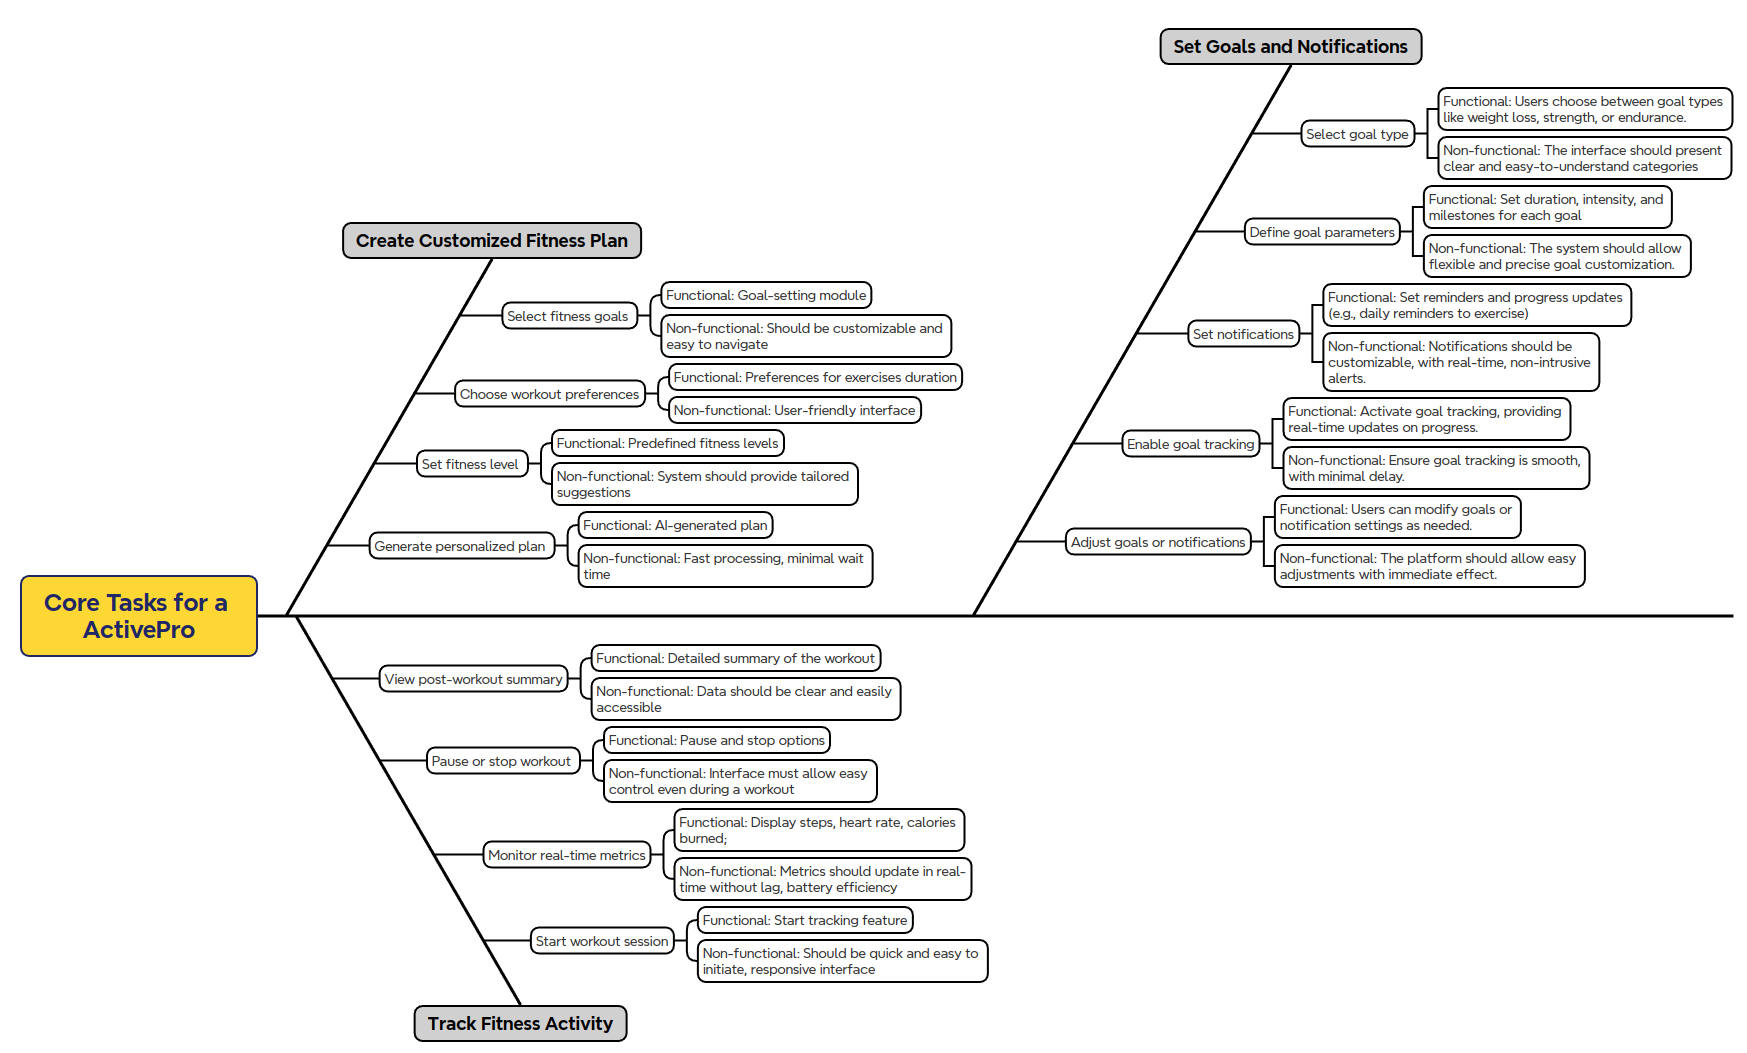
\includegraphics[width=18cm, height=12cm]{image3}
\end{figure}



%----------------------------------------------------------------------------------------

\end{document}